\chapter{Теоретические основы каскадирования}

Вычислительные эксперименты, проводимые с целью исследования каскадных разделительных схем, опираются на использование специальных математических моделей, которые будут представлены в текущем разделе. Они позволяют заметно упростить изучение закономерностей изотопно-селективного массопереноса в разделительных каскадах. Этот вспомогательный инструмент принято называть модельным каскадом.

Важно отметить, что физико-математические модели каскадов основаны на фундаментальных законах, таких как закон сохранения вещества и эти теоретические описания адекватны процессу разделения в реальных каскадах, состоящих из тысяч разделительных аппаратов (в качестве которых сегодня, как правило, используют газовые центрифуги).

Тогда как обогащение природного урана можно свести к простой задаче разделения бинарной смеси, обогащение регенерированного урана является задачей разделения изотопов многокомпонентной изотопной смеси. Отсюда, сложность расчетов молекулярно-селективного переноса для многокомпонентных изотопных составов заключается в необходимости использования математических моделей для разделения многокомпонентных изотопных смесей.

\section{Основы теории разделения в каскадах}

На сегодняшний день разработан обширный набор расчетных моделей, которые могут быть применены в том числе и к задаче обогащения регенерированного урана \cite{smirnovMolekulyarnoselektivnyyMassoperenosKomponentov2013}. Введем основные теоретические понятия и рассмотрим модельные каскады, релевантные задаче диссертационной работы.

\subsection{Понятие разделительной ступени}

Ниже рассмотрены общие характеристики разделительных ступеней, предназначенных для разделения многокомпонентных изотопных смесей в газовой фазе. В качестве разделяемой смеси рассмотрена смесь, содержащая \textit{m} химически не реагирующих между собой компонентов, содержание которых будем определять их мольными долями (концентрациями) $C_{i}$ ($i=1,\, 2,...,m$) \cite{sulaberidzeTeoriyaKaskadovDlya2011}. Компоненты пронумерованы в порядке возрастания массовых чисел. Для концентраций компонентов разделяемой смеси справедливо очевидное тождество:

\begin{equation} \label{GrindEQ__1_1_} 
  \sum _{j=1}^{m}C_{j}  =1 
\end{equation} 
  
Как правило, вместо концентраций $C_{i} $, используют относительные концентрации, определяемые по отношению к концентрации так называемого «опорного» компонента с фиксированным номером, например, \textit{k}, то есть

\begin{equation} \label{GrindEQ__1_2_} 
  R_{ik} =\frac{C_{i} }{C_{k} } , i=1,\, 2,...,m.             
\end{equation} 
  
В качестве <<опорного>> может быть выбран любой из компонентов смеси, всего имеется   таких наборов. 
Простая разделительная ступень имеет один входной поток и два выходных (рис. \ref{1_1}). На вход ступени поступает поток питания (производительность ступени) $L$  (в моль/с) с концентрациями $C_{i}$ ($i=1,\, 2,...,m$). Из ступени выходят два потока: легкая фракция (поток, обогащенный легкими компонентами) или отбор ступени $L'$ и тяжелая фракция (поток, обедненный легкими компонентами) или отвал ступени $L''$. Концентрации компонентов в этих потоках  $C'_{i} $ и $C''_{i} $  соответственно.

\begin{figure}[ht]
  \centerfloat{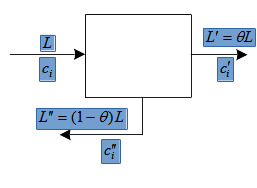
\includegraphics[scale=0.7]{images/theory/lu15087t0po}}
  \caption{Схема разделительной ступени }\label{1_1}
\end{figure}

Коэффициент деления потоков смеси (срез) $\theta$, парциальные потоки компонентов $G_{i} ,\; G'_{i} ,\; G''_{i}$ и срезы парциальных потоков $\phi _{i}$ можно определить по формулам:

\begin{equation} \label{GrindEQ__1_3_} 
  \theta =\frac{L'}{L} ,\; G_{i} =LC_{i} ,\; G'_{i} =L'C'_{i} ,\; G''_{i} =L''C''_{i} , 
  \end{equation} 
  \begin{equation} \label{GrindEQ__1_4_} 
  \phi _{i} =\frac{G'_{i} }{G_{i} } ,\; 1-\phi _{i} =\frac{G"_{i} }{G_{i} } ,\; i=1,2,...,m. 
  \end{equation} 

Уравнения баланса ступени в стационарном режиме работы и в отсутствие потерь рабочего вещества имеют вид:

\begin{equation} \label{GrindEQ__1_5_} 
  L=L'+L'', 
  \end{equation} 
  \begin{equation} \label{GrindEQ__1_6_} 
  G_{i} =G'_{i} +G''_{i} , i=1,\, 2,...,m.             
\end{equation} 
  

Введенное в \ref{GrindEQ__1_3_} определение среза потоков ступени дает возможность представить уравнения \ref{GrindEQ__1_6_} в следующем виде:

\begin{equation} \label{GrindEQ__1_7_} 
  C_{i} =\theta C'_{i} +(1-\theta )C''_{i} . 
\end{equation} 

Из \ref{GrindEQ__1_5_} и \ref{GrindEQ__1_6_} непосредственно следует:

\begin{equation} \label{GrindEQ__1_8_} 
  L=\sum _{j=1}^{m}G_{j}  ,\; \; L'=\sum _{j=1}^{m}G'_{j} ,\; \;  L''=\sum _{j=1}^{m}G''_{j} ,\; \;   
  \end{equation} 
  \begin{equation} \label{GrindEQ__1_9_} 
  C_{i} =\frac{G_{i} }{\sum _{j=1}^{m}G_{j}  } ,\; \; C'_{i} =\frac{G'_{i} }{\sum _{j=1}^{m}G'_{j}  } ,\; \; C''_{i} =\frac{G''_{i} }{\sum _{j=1}^{m}G''_{j}  } , i=1,\, 2,...,m,             
  \end{equation} 
  \begin{equation} \label{GrindEQ__1_10_} 
  \theta =\frac{\sum _{j=1}^{m}G'_{j}  }{\sum _{j=1}^{m}G_{j}  } .            
\end{equation} 

Для каждого компонента $i$ с относительной концентрацией $R_{ik}$ вводят относительные коэффициенты разделения: полный $q_{ik}$, в отборе $\alpha _{ik} $ и в отвале $\beta _{ik} $ и соответствующие коэффициенты обогащения $\varepsilon _{ik} ,\varepsilon '_{ik} ,\; \varepsilon ''_{ik} \; $
\[q_{ik} =\frac{R'_{ik} }{R''_{ik} } ,\; \; \alpha _{ik} =\frac{R'_{ik} }{R_{ik} } ,\; \; \beta _{ik} =\frac{R_{ik} }{R''_{ik} } ,\] 

\begin{equation} \label{GrindEQ__1_11_} 
  \begin{array}{l}
    \qquad q_{i k}=\frac{R_{i k}^{\prime}}{R_{i k}^{\prime \prime}}, \alpha_{i k}=\frac{R_{i k}^{\prime}}{R_{i k}}, \beta_{i k}=\frac{R_{i k}}{R_{i k}^{\prime \prime}} \\
    \varepsilon_{i k}=q_{i k}-1, \varepsilon_{i k}^{\prime}=\alpha_{i k}-1, \varepsilon_{i k}^{\prime \prime}=1-\frac{1}{\beta_{i k}}
    \end{array}
\end{equation} 

При разделении изотопов молекулярно-кинетическими методами величины относительных коэффициентов разделения можно аппроксимировать соотношениями $q_{ij} =q_{0} {}^{M_{j} -M_{i} }$, где \textit{q}${}_{0}$ – коэффициент разделения, приходящийся на единицу разности массовых чисел; \textit{M${}_{i}$, M${}_{j}$} – массовые числа $i$-го и $j$-го компонентов, соответственно \cite{sulaberidzeTeoriyaKaskadovDlya2011}.

При фиксированном номере «опорного» компонента (в качестве «опорного» выбран компонент с номером $k$) существует набор из ($m-1$) независимых $q_{ik} $ (или $\alpha _{ik} $, $\beta _{ik}$). По определению $R_{ik} $ имеется $m$ таких наборов. Однако, каждый из них, например $q_{ik} $, может быть преобразован в другой набор, например, $q_{ij}$ по формулам

\begin{equation} \label{GrindEQ__1_12_} 
  q_{ij} =q_{ik} \cdot q_{kj} .            
\end{equation} 

Если $k\ne m$, то при всех $i<k$ значения всех коэффициентов разделения $q_{ik} $, $\alpha _{ik} $, $\beta _{ik} $, будут больше единицы, а при всех $i>k$ -- меньше единицы.

Полные коэффициенты разделения $q_{ik} $, как правило, не зависят от состава смеси. В некоторых случаях, что характерно для газовой центрифуги, коэффициенты $q_{ik} $ могут зависеть от коэффициента деления потоков смеси (срез) $\theta $. Так, в общем случае, для газовой центрифуги, полный коээфициент разделения зависит также от коэффициента деления потоков смеси (срез) $\theta$ и от потока питания на один разделительный элемент ступени $g_{s} $ (\ref{GrindEQ__q_}) \cite{mustafinObjectiveFunctionOptimization2019}:

\begin{equation} \label{GrindEQ__q_} 
  q_{ij} = f(\theta, g_{s}),              
\end{equation}

Введем обозначения:

\begin{equation} \label{GrindEQ__1_13_} 
  g_{i} =\frac{\phi _{i} }{1-\phi _{i} } =\frac{G'_{i} }{G''_{i} } , i\ne k, 
  \end{equation} 
  \begin{equation} \label{GrindEQ__1_14_} 
  g_{k} =\frac{\phi _{k} }{1-\phi _{k} } =\frac{G'_{k} }{G''_{k} } .           
\end{equation} 

Нетрудно показать, используя  \ref{GrindEQ__1_9_} и  \ref{GrindEQ__1_11_}, что величины $g_{i}$ и $g_{k}$  связаны с величинами относительных коэффициентов разделения следующими соотношениями:

\begin{equation} \label{GrindEQ__1_15_} 
  g_{i} =\frac{\alpha _{ik} (\beta _{ik} -1)}{\alpha _{ik} -1} ,\; \; i\ne k,           
  \end{equation} 
  \begin{equation} \label{GrindEQ__1_16_} 
  g_{k} =\frac{\beta _{ik} -1}{(\alpha _{ik} -1)\beta _{ik} } =\frac{\varepsilon ''_{ik} }{\varepsilon '_{ik} } . 
\end{equation} 

При этом

\begin{equation} \label{GrindEQ__1_17_} 
  \frac{g_{i} }{g_{k} } =q_{ik} .           
\end{equation} 

С использованием выражений \ref{GrindEQ__1_1_}--\ref{GrindEQ__1_17_} получим следующие соотношения, связывающие параметры отдельной ступени каскада

\begin{equation} \label{GrindEQ__1_18_} 
  L=\sum _{j=1}^{m}L_{i}  =\sum _{j=1}^{m}\frac{g_{i} +1}{g_{i} }  L_{i} ',               
  \end{equation} 
  \begin{equation} \label{GrindEQ__1_19_} 
  C_{i} =\frac{g_{i} +1}{g_{i} } \frac{L_{i} '}{L} ,         
  \end{equation} 
  \begin{equation} \label{GrindEQ__1_20_} 
  \theta =\frac{L^{'} }{L} ={\sum _{j=1}^{m}L_{j}^{'}  \mathord{\left/ {\vphantom {\sum _{j=1}^{m}L_{j}^{'}   \sum _{j=1}^{m}L_{j}  }} \right. \kern-\nulldelimiterspace} \sum _{j=1}^{m}L_{j}  } .      
\end{equation} 

\subsection{Симметричный противоточный каскад и система уравнений, описывающих для него массоперенос в общем виде}

Среди различных способов коммутации ступеней в разделительных каскадах наиболее распространенным является так называемый способ симметричного соединения ступеней в противоточной схеме (рис. \ref{1_2}). Рассмотрим схему такого каскада, имеющего один входящий поток питания $F$ и два выходящих: отбор $P$, обогащенный самым легким компонентом и отвал W, обогащенный самым тяжелым компонентом. Потоки $F$, $P$, $W$ и концентрации компонентов в них $C_{i}^{F} ,\; \; C_{i}^{P} ,\; \; C_{i}^{W} \; \; (i=1,\; 2,...,m)$ являются внешними параметрами каскада. Следует заметить, что в случае разделения многокомпонентных смесей понятия «отбор» и «отвал» условны, поскольку ценный компонент может обогащаться как вместе с самым легким компонентом смеси, так и вместе с самым тяжелым.

\begin{figure}[ht]
  \centerfloat{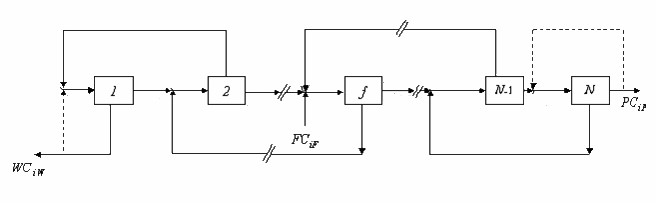
\includegraphics[scale=0.7]{images/theory/2}}
  \caption{Схема соединения ступеней в симметрично-противоточном каскаде}\label{1_2}
\end{figure}

В отсутствие потерь рабочего вещества на ступенях каскада, внешние параметры каскада должны удовлетворять уравнениям материального баланса

\begin{equation} \label{GrindEQ__1_21_} 
  \begin{array}{l} {\quad \quad \quad \quad F=P+W,} \\ {FC_{i}^{F} =PC_{i}^{P} +WC_{i}^{W} ,\; i=1,2,...,m.} \end{array} 
\end{equation} 

Ступени каскада пронумерованы последовательно от $s=1$ на отвальном конце каскада до $s=N$ на отборном конце. Считаем, что внешнее питание каскада (\textit{F}) подают на вход ступени с номером $f$. Внутренние параметры произвольной ступени с номером \textit{s} ($L_{s} $, $L'_{s} ,$ $L''_{s} ,$ $G_{i,s} ,$ $G'_{i,s} ,$ $G''_{i,s} $), где $L$ -- потоки вещества, а $G$ -- парциальные потоки (изотопов с индексами $i$) в стационарном режиме работы каскада, в отсутствие потерь рабочего вещества на ступенях каскада, согласно  \ref{GrindEQ__1_5_},  \ref{GrindEQ__1_6_} связаны уравнениями баланса вещества и каждого компонента

\begin{equation} \label{GrindEQ__1_22_} 
  L_{s} =L'_{s} +L''_{s} ,\; \; s=1,...,N,            
  \end{equation} 
  \begin{equation} \label{GrindEQ__1_23_} 
  G_{i,s} =G'_{i,s} +G''_{i,s} ,\;s=1,...,N \; i=1,2,...,m.           
  \end{equation} 

где индекс $i$ означает номер компонента.

Уравнения баланса в «узлах» (точках соединения межступенных потоков) при симметричном соединении ступеней имеют вид:

\begin{equation} \label{GrindEQ__1_24_} 
  L_{s} =\theta _{s-1} L_{s-1} +(1-\theta _{s+1} )L_{s+1} ,\; \; s=1,\, 2,...,f-1,\, f+1,...,N, 
  \end{equation} 
  \begin{equation} \label{GrindEQ__1_25_} 
  \begin{array}{l} {L_{s} C_{i,s} =\theta _{s-1} L_{s-1} C'_{i,s-1} +(1-\theta _{s+1} )L_{s+1} C''_{i,s+1} ,\; \; s=1,\, 2,...,f-1,\, f+1,...,N,} \\ {\; \; \; \; \; \; \; \; \; \; \; \; \; \; \; \; \; \; \; \; \; \; \; \; \; \; \; \; \; \; \; \; \; \quad \quad \quad \quad \quad \; \; \; \; \; \; \; \; \; \; \; \; \; \quad \quad \quad \; \; \; \; \; \; \; \; \; \; \; \; \; \quad \quad \quad \; \; \; \; \; \; \; \; \; \; \; \; \; \quad \quad \; \quad i=1,\, 2,...,m.} \end{array} 
  \end{equation} 

Для ступени подачи питания $f$ аналогичные уравнения выглядят так:

\begin{equation} \label{GrindEQ__1_26_} 
  L_{f} =\theta _{f-1} L_{f-1} +(1-\theta _{f+1} )L_{f+1} +F, 
  \end{equation} 
  \begin{equation} \label{GrindEQ__1_27_} 
  L_{f} C_{i,f} =\theta _{f-1} L_{f-1} C'_{i,f-1} +(1-\theta _{f+1} )L_{f+1} C''_{i,f+1} +FC_{i}^{F} ,\quad i=\overline{1,m}.            
\end{equation}

Внешние и внутренние параметры каскада связаны граничными условиями

\begin{equation} \label{GrindEQ__1_28_} 
  L_{0} =L'_{0} =L''_{0} =L_{N+1} =L'_{N+1} =L''_{N+1} =0, 
  \end{equation} 
  \begin{equation} \label{GrindEQ__1_29_} 
  L'_{N} =\theta _{N} L_{N} =P,        
  \end{equation} 
  \begin{equation} \label{GrindEQ__1_30_} 
  L''_{1} =(1-\theta _{1} )L_{1} =W,        
  \end{equation} 
  \begin{equation} \label{GrindEQ__1_31_} 
  C'_{N} =C_{i}^{P} ,\; i=1,\; \; 2,...,m, 
  \end{equation} 
  \begin{equation} \label{GrindEQ__1_32_} 
  C''_{1} =C_{i}^{W} ,\; i=1,\; \; 2,...,m, 
  \end{equation} 
  \begin{equation} \label{GrindEQ__1_33_} 
  G'_{i,N} =PC_{i}^{P} ,\; i=1,\; \; 2,...,m, 
  \end{equation} 
  \begin{equation} \label{GrindEQ__1_34_} 
  G''_{i,1} =WC_{i}^{W} ,\; i=1,\; \; 2,...,m. 
\end{equation} 

Соотношения (\ref{GrindEQ__1_21_})--(\ref{GrindEQ__1_34_}) описывают простейшую физико-математическую модель противоточного симметричного каскада, предназначенного для разделения многокомпонентной смеси. При решении некоторых разделительных задач вместо уравнений (\ref{GrindEQ__1_24_})--(\ref{GrindEQ__1_27_}) удобнее пользоваться разностными уравнениями, отражающими баланс потоков в сечениях между ступенями:

для обогатительной части каскада:

\begin{equation} \label{GrindEQ__1_35_} 
  \theta _{s} L_{s} -(1-\theta _{s+1} )L_{s+1} =P, 
  \end{equation} 
  \begin{equation} \label{GrindEQ__1_36_} 
  \theta _{s} L_{s} C'_{i,s} -(1-\theta _{s+1} )L_{s+1} C''_{i,s+1} =PC_{i}^{P} \; \; i=1,\, 2,...,m,        
  \end{equation} 

для обеднительной части каскада:

\begin{equation} \label{GrindEQ__1_37_} 
  \theta _{s} L_{s} -(1-\theta _{s+1} )L_{s+1} =-W, 
  \end{equation} 
  \begin{equation} \label{GrindEQ__1_38_} 
  \theta _{s} L_{s} C'_{i,s} -(1-\theta _{s+1} )L_{s+1} C''_{i,s+1} =-WC_{i}^{W} \; i=1,\; \; 2,...,\; m.        
  \end{equation} 

Величины, стоящие в левых частях уравнений (\ref{GrindEQ__1_35_})--(\ref{GrindEQ__1_38_}), как правило, называют «транзитными» потоками смеси в целом (уравнения (\ref{GrindEQ__1_35_}) и (\ref{GrindEQ__1_37_})) и ее отдельных компонентов (уравнения (\ref{GrindEQ__1_36_}) и (\ref{GrindEQ__1_38_})) \cite{sulaberidzeTeoriyaKaskadovDlya2011}. С физической точки зрения указанные уравнения определяют величину количества переносимого вещества в направлении от отвала к отбору. Отметим, что, в случае необходимости, аналогичные уравнения могут быть получены и для переноса вещества в направлении от отбора к отвалу. 
В свою очередь система (\ref{GrindEQ__1_35_})--(\ref{GrindEQ__1_38_}) может быть легко преобразована к виду:

\begin{equation} \label{GrindEQ__1_39_} 
  C_{i,s+1} -C_{i,s} =\frac{\theta _{s} L_{s} }{(1-\theta _{s+1} )L_{s+1} } \delta '_{i,s} +\delta ''_{i,s+1} -\frac{P\left(C_{i}^{P} -C_{i,s} \right)}{(1-\theta _{s+1} )L_{s+1} } ,        
  \end{equation} 

\[i=1,\, 2,...,m;\; \; s=f,...,N,\] 

, где $\delta '_{i,s} =C'_{i,s} -C_{i,s} $ -- функция, представляющая собой изменение концентрации $i$-го компонента в потоке обогащенной фракции $s$-й ступени; $\delta ''_{i,s} =C_{i,s} -C''_{i,s} $ – функция, представляющая собой изменение концентрации i-го компонента в потоке обедненной фракции $s$-й ступени.

Соответственно, система (\ref{GrindEQ__1_35_})--(\ref{GrindEQ__1_38_}) может быть представлена в виде

\begin{equation} \label{GrindEQ__1_40_} 
  C_{i,s+1} -C_{i,s} =\frac{\theta _{s} L_{s} }{(1-\theta _{s+1} )L_{s+1} } \delta '_{i,s} +\delta ''_{i,s+1} -\frac{W(C_{i,s} -C_{i}^{W} )}{(1-\theta _{s+1} )L_{s+1} } ,        
  \end{equation} 
  \[i=1,\, 2,...,m;\; \; s=1,\, 2,...,f-1.\] 

Отметим, что системы (\ref{GrindEQ__1_24_})--(\ref{GrindEQ__1_27_}), (\ref{GrindEQ__1_35_})--(\ref{GrindEQ__1_38_}) и (\ref{GrindEQ__1_39_})--(\ref{GrindEQ__1_40_}) эквивалентны. Анализ данных систем показывает, что они обе представляют собой системы нелинейных разностных уравнений относительно функций $C_{i,s}$. Существенной проблемой при решении подобных систем является то, что в эти уравнения (либо в их граничные условия) входят значения концентраций, которые неизвестны заранее и должны быть определены из решения этих же уравнений. Аналитическое решение подобных систем удается найти лишь для некоторых частных случаев (данные случаи рассмотрены ниже) \cite{sulaberidzeTeoriyaKaskadovDlya2011}. В общем случае, системы (\ref{GrindEQ__1_24_})--(\ref{GrindEQ__1_27_}), (\ref{GrindEQ__1_35_})--(\ref{GrindEQ__1_38_}) или (\ref{GrindEQ__1_39_})--(\ref{GrindEQ__1_40_}) требуют использования численных методов. При этом, как правило, выделяют 2 типа задач расчета параметров каскада: поверочный расчет и проектировочный расчет.

Под поверочным расчетом каскада подразумевают следующую задачу:
Задано: состав исходной разделяемой смеси,  число ступеней в каскаде и величины питающих их потоков, величины внешнего потока питания и одного из выходящих потоков каскада (отбора или отвала), параметры ступени (например, относительные коэффициенты разделения ступеней и др.).
Подлежат определению: концентрации всех компонентов в потоках отбора  и отвала и распределение концентраций компонентов по ступеням каскада. 
Поверочный расчет каскада необходим при исследовании оптимального управления процессом разделения, при изменении режимов работы и отдельных параметров разделительного каскада \cite{sulaberidzeTeoriyaKaskadovDlya2011}. Основные трудности поверочного расчета связаны с тем, что неизвестные концентрации компонентов в потоках отбора и отвала сами явно входят в основные уравнения переноса (или их граничные условия). Невозможность аналитического решения этих уравнений вызывает необходимость разработки численных методов, малочувствительных к заданию начальных приближений для концентраций компонентов в выходящих потоках. На сегодняшний день предложены различные методы поверочного расчета, которые позволяют численно решить данную задачу \cite{sulaberidzeTeoriyaKaskadovDlya2011, sazykinUsovershenstvovannyyMetodRascheta1997, wuCalculationMethodsDetermining1988, holpanovEffektivnyyMetodRascheta1998, potapovCalculationSquaredoffCascades1996, zengRobustEfficientCalculation2000}.

Под проектировочным расчетом каскада обычно подразумевают следующую задачу \cite{sulaberidzeTeoriyaKaskadovDlya2011}.
Задано: состав исходной разделяемой смеси, один из выходящих потоков каскада (отбор или отвал), концентрации одного из компонентов (целевого или ключевого) в потоках отбора и отвала.
Подлежат определению: все внутренние параметры каскада (распределение потока и концентраций компонентов по ступеням каскада и др.), концентрации остальных компонентов (всех кроме ключевого) в потоках отбора и отвала. 
При этом, очевидно, что найденные параметры каскада должны соответствовать оптимальным условиям разделения в каскаде.

Трудности решения (\ref{GrindEQ__1_24_})--(\ref{GrindEQ__1_27_}), (\ref{GrindEQ__1_35_})--(\ref{GrindEQ__1_38_}) и (\ref{GrindEQ__1_39_})--(\ref{GrindEQ__1_40_}) в общем случае, стимулировали развитие упрощенных подходов, которые позволяют получить аналитическое решение для данных систем при введении определенных предположений. Полученные в результате таких упрощений физико-математические модели симметрично-противоточного каскада сохраняют закономерности молекулярно-селективного массопереноса, но позволяют заметно упростить соответствующие расчетные процедуры для определения оптимальных параметров каскада. Такие каскады получили название модельных \cite{minenkoTeoriiKaskadovDlya1965, delagarzaMulticomponentIsotopeSeparation1961, zhigalovskiyLekcionnyeMaterialyPo1999, kolokoltsovDesignCascadesSeparating1970, kolokolcovVoprosuPostroeniiKaskadov1970, minenkoPredelnoeObogashcheniePromezhutochnyh1972, yamamotoMulticomponentIsotopeSeparating1978, wuStudyMulticomponentIsotope, borisevichRascheteKaskadovDopolnitelnym1993, woodCriterionEffiencyMultiisotope1999, sulaberidzeOsobennostiObogashcheniyaKomponentov2006, sazykinKvaziidealnyeKaskadyDlya2000, sulaberidzeSravnenieOptimalnyhModelnyh2008}.

Целесообразной областью применения теории модельных каскадов является ее использование при предварительном рассмотрении актуальных проблем современной теории разделения многокомпонентных изотопных смесей в каскадах и смежных с разделительной наукой областей, таких, например, как ядерная энергетика. В рамках данной работы анализ строится на основе теории модельных каскадов, однако выявленные физические закономерности массопереноса в рассмотренных каскадных схемах справедливы и в близких к реализуемых в производственных условиях прямоугольных и прямоугольно секционированных каскадов.

Так и в рамках данной диссертации, для моделирования физического процесса разделения изотопов урановой смеси может быть применен целый ряд из таких специальных математических моделей, из которых будет выбран R-каскад. Такой выбор был сделан ввиду того, что основной целью проведения вычислительных экспериментов являлись расчет изотопных составов получаемого в схеме конечного продукта (товарного низкообогащенного урана) и оценка ключевых интегральных параметров каскадных схем (массовые расходы регенерата и обедненного урана, потоки между каскадами, затраты работы разделения и другие), при этом R-каскады характеризуются параметрами, близкими к параметрам каскадов, оптимизированных по величине суммарного потока. Последнее обстоятельство фактически означает минимальность затрат работы разделения в случае обогащения регенерированного урана. 

Далее рассмотрим подробнее математические модели, нашедшие свое применение в расчетных исследованиях данной диссертации.

Наиболее общая из таких моделей называется «квазиидеальным» каскадом, где предполагается постоянство по всей его длине относительных коэффициентов разделения, а также срезов парциальных компонентов по каскадным ступеням \cite{yamamotoMulticomponentIsotopeSeparating1978}.
В настоящее время он используется в двух приближениях: со слабым обогащением (Q-каскад \cite{borisevichNewApproachOptimize2011, kolokoltsovDesignCascadesSeparating1970, zengQCascadeExplanation2012}) и произвольным обогащением (квазиидеальный каскад \cite{sulaberidzeSpecialFeaturesEnrichment2006}).
Применение модельных каскадов значительно упрощает как анализ закономерностей массообмена в каскаде для многокомпонентного разделения, так и соответствующий расчет.
В исследованиях, как правило, когда обогащенный переработанный уран обогащается многопоточными схемами, часто используется модель R-каскада (Matched Abundance Ratio Cascade-MARC \cite{kazukihidaSimultaneousEvaluationEffects1986, delagarzaMulticomponentIsotopeSeparation1961, woodEffectsSeparationProcesses2008}).
Это особый случай `квазиидеального' каскада. Здесь условие отсутствия смешивания концентраций при подаче в каждую ступень выполняется для выбранной пары компонентов (например, это могут быть изотопы $^{235}$U и $^{238}$U).
Еще раз подчеркнем, что все вышеупомянутые каскадные модели действуют как физически эквивалентные представления и, как показано в \cite{sulaberidzeClassificationModelCascades2020}, могут быть выведены из <<обобщенного модельного каскада>>, которым является симметрично-противоточный каскад с постоянными по его длине относительными коэффициентами разделения).

Работе по поиску схем для обогащения регенерата предшествовали разработки математического аппарата для моделирования разделения многокомпонентных смесей \cite{delagarzaMulticomponentIsotopeSeparation1961}.
Изначально, эту идею рассматривали для газодиффузионного метода разделения, которая в последующем была адаптирована для метода газовой центрифуги с характерными большими коэффициентами разделения \cite{yamamotoMulticomponentIsotopeSeparating1978}.

Последовательно проходя через основные вехи развития модельных каскадов для моделирования многокомпонентных изотопных смесей, в работе \cite{delagarzaMulticomponentIsotopeSeparation1961} предложена модель R-каскада, а в \cite{levin1963} -- М*-каскада.
Затем в \cite{kolokoltsovDesignCascadesSeparating1970} разработана модель Q-каскада, а в \cite{sazykinKvaziidealnyeKaskadyDlya2000} -- квазиидеального.

Ниже кратко рассмотрены модельные каскады, для интересующего нас случая произвольного немалого коэффициента разделения на ступенях -- «квазиидеальный» каскад и его частный случай R-каскад \cite{sazykinKvaziidealnyeKaskadyDlya2000}.

\subsection{Модель «квазиидеального» каскада}

Рассмотрим случай симметричного противоточного каскада с постоянными по его длине относительными коэффициентами разделения $q_{ik} ,\; \alpha _{ik} ,\; \beta _{ik} $ $(i=1,\; 2,...,m;$ \textit{k}--номер «опорного» компонента). Условие постоянства относительных коэффициентов разделения обеспечивает выполнение условия постоянства величин \textit{g${}_{i}$} и $\phi _{i} $. Следовательно, соотношения (\ref{GrindEQ__1_24_})--(\ref{GrindEQ__1_27_}) приводятся к виду \cite{sulaberidzeTeoriyaKaskadovDlya2011}:

\begin{equation} \label{GrindEQ__1_52_} 
  G'_{i} (s-1)+\frac{1}{g_{i} } G'_{i} (s+1)-\frac{g_{i} +1}{g_{i} } G'_{i} (s)+\delta _{sf} Fc_{iF} =0,\; \; i\ne k, 
  \end{equation} 
  \begin{equation} \label{GrindEQ__1_53_} 
  G'_{k} (s-1)+\frac{1}{g_{k} } G'_{k} (s+1)-\frac{g_{k} +1}{g_{k} } G'_{k} (s)+\delta _{sf} Fc_{kF} =0, 
  \end{equation}

где $s$ – текущий номер ступени, отсчитываемый от «тяжелого» конца каскада к его «легкому» концу $\delta _{sf} =\left\{\begin{array}{l} {0,\; \; s\ne f} \\ {1,\; \; s=f} \end{array}\right. $

Уравнения (\ref{GrindEQ__1_52_})--(\ref{GrindEQ__1_53_}) представляют собой линейные разностные уравнения второго порядка относительно неизвестных функций $G'_{i} (s)$. Граничные условия для них имеют вид:

\begin{equation} \label{GrindEQ__1_54_} 
  \left\{\begin{array}{l} {G'_{i} (0)=G'_{i} (N+1)=0,\; \; i=1,\; 2,...,m} \\ {G'_{i} (N)=PC_{i}^{P} ,\; \; i=1,\; 2,...,m} \\ {G'_{i} (1)=g_{i} WC_{i}^{W} ,\; \; i\ne k} \\ {G''_{k} (1)=g_{k} WC_{i}^{W} .} \end{array}\right.  
\end{equation} 

Ступени с номерами $s=1$ и $s=N$ являются крайними ступенями каскада, что делает возможным формально записать $G'_{i} (0)=G'_{i} (N+1)=0$.

Решив (\ref{GrindEQ__1_52_}) и (\ref{GrindEQ__1_53_}), а также используя уравнения баланса (\ref{GrindEQ__1_21_}) и граничные условия (\ref{GrindEQ__1_54_}), можно получить уравнения связи внешних параметров такого каскада с длинами его секций и параметрами ступени. В итоге:

\begin{equation} \label{GrindEQ__1_55_} 
  \frac{P}{F} =\sum _{j=1}^{m}C_{j}^{F} \frac{1-g_{j}^{-f} }{1-g_{j}^{-N-1}} ,\; \; s=f,...,N ,                                                  
  \end{equation} 
  \begin{equation} \label{GrindEQ__1_56_} 
  \frac{W}{F} =\sum _{j=1}^{m}C_{j}^{F} \frac{g_{j}^{N+1-f} -1}{g_{j}^{N+1} -1} ,\; \; s=1,...,f-1 ,                                            
\end{equation}

\begin{equation} \label{GrindEQ__1_57_} 
  C_{i}^{P}=C_{i}^{F} \frac{1-g_{i}^{-f}}{1-g_{i}^{-N-1}} / \sum_{j=1}^{m} C_{j}^{F} \frac{1-g_{j}^{-f}}{1-g_{j}^{-N-1}}, i=1,2, \ldots, m                             
\end{equation}

\begin{equation} \label{GrindEQ__1_58_} 
  C_{i}^{W}=C_{i}^{F} \frac{g_{i}^{N+1-f}-1}{g_{i}^{N+1}-1} / \sum_{j=1}^{m} C_{j}^{F} \frac{g_{j}^{N+1-f}-1}{g_{j}^{N+1}-1}, i=1,2, \ldots, m                         
\end{equation} 

Далее, распределение потока $L(s)$, концентраций компонентов и коэффициента деления потоков по ступеням каскада можно определить по формулам \cite{sulaberidzeTeoriyaKaskadovDlya2011}:

\begin{equation} \label{GrindEQ__1_59_} 
L(s)=\sum_{j=1}^{m} G_{j}^{\prime}(s) \frac{1+g_{j}}{g_{j}}=\left\{\begin{array}{c}
  P \sum_{j=1}^{m} \frac{g_{j}+1}{g_{j}-1} C_{j}^{P}\left(1-g_{j}^{s-N-1}\right), s=f, \ldots, N \\
  W \sum_{j=1}^{m} \frac{g_{j}+1}{g_{j}-1} C_{j}^{\pi}\left(g_{j}^{s}-1\right), s=1, \ldots, f-1
  \end{array}\right.
\end{equation} 

\begin{equation} \label{GrindEQ__1_60_} 
C_{i} (s)=\frac{1+g_{j} }{g_{j} } \cdot \frac{G''_{i} (s)}{G_{i} (s)} =\left\{\begin{array}{l} {\frac{C_{i}^{P} \frac{g_{j} }{g_{j} -1} \left(1-g_{j}^{s-N-1} \right)}{\sum _{j=1}^{m}\frac{g_{j} +1}{g_{j} -1}  C_{j}^{P} \left(1-g_{j}^{s-N-1} \right)} ,\; \; s=f,...,N,} \\ {\; \frac{C_{i}^{W} \frac{g_{j} }{g_{j} -1} \left(g_{j}^{s} -1\right)}{\sum _{j=1}^{m}\frac{g_{j} +1}{g_{j} -1}  C_{j}^{W} \left(g_{j}^{s} -1\right)} ,\; \; s=1,...,f-1,} \end{array}\right.  
\end{equation} 

\begin{equation} \label{GrindEQ__1_61_} 
\begin{array}{l} {\theta (s)=\frac{\sum _{j=1}^{m}G'_{j} (s) }{\sum _{j=1}^{m}G_{j} (s) } =\left\{\begin{array}{l} {\frac{\sum _{j=1}^{m}\frac{g_{j} }{g_{j} -1} C_{j}^{P} \left(1-g_{j}^{s-N-1} \right) }{\sum _{j=1}^{m}\frac{g_{j} +1}{g_{j} -1}  C_{j}^{P} \left(1-g_{j}^{s-N-1} \right)} ,\; \; s=f,...,N,} \\ {\; \frac{\sum _{j=1}^{m}\frac{g_{j} }{g_{j} -1} C_{j}^{W} \left(g_{j}^{s} -1\right) }{\sum _{j=1}^{m}\frac{g_{j} +1}{g_{j} -1}  C_{j}^{W} \left(g_{j}^{s} -1\right)} ,\; \; s=1,...,f-1.} \end{array}\right. } \\ {\; } \end{array} 
\end{equation}

Формулу для расчета относительного суммарного потока в каскаде легко получить, суммируя (\ref{GrindEQ__1_59_}) по всем ступеням каскада

\begin{equation} \label{GrindEQ__1_62_} 
  \sum _{s=1}^{N}\frac{L(s)}{P} =\sum _{i=1}^{m}\left\{\frac{g_{i} +1}{g_{i} -1} \left[\frac{W}{P} C_{i}^{W} (f)+C_{i}^{P} \left(N+1-f\right)\right]\right\}  .   
\end{equation} 
  
Рассмотренный выше каскад отличается тем, что относительные коэффициенты разделения $q_{ik} ,\; \alpha _{ik} ,\; \beta _{ik} $ (и, соответственно, срезы парциальных компонентов $\phi _{i} ,\; \; \phi _{k} $ и параметры $g_{i} $, $g_{k} $) остаются постоянными по длине каскада. Для таких каскадов в работе \cite{sazykinKvaziidealnyeKaskadyDlya2000} был введен термин «квазиидеальный» каскад.

\subsection{Каскад с несмешиванием относительных концентраций двух заданных компонентов смеси (R-каскад)}

Рассмотрим R-каскад, в котором выполняется несмешивание относительных концентраций $n$-го и $k$-го компонентов смеси. Данная каскадная модель является аналогом используемого в теории разделения бинарных смесей «идеального» каскада, в «узлы» которого входят потоки с одинаковой концентрацией компонентов. R-каскады могут быть построены как в случае «слабого обогащения», так и для немалых обогащений на ступени. Рассмотрим R-каскад в случае немалых обогащений на ступени. Условие несмешения по относительным концентрациям $n$-го и $k$-го компонентов можно записать в виде:

\begin{equation} \label{GrindEQ__1_68_} 
  R'_{nk} (s-1)=R_{nk} (s)=R''_{nk} (s+1).                                                 
\end{equation} 

Вследствие (\ref{GrindEQ__1_68_}) коэффициенты $\alpha _{nk} $ и $\beta _{nk} $ совпадают для двух соседних ступеней. При постоянных полных коэффициентах разделения равенство:

\begin{equation} \label{GrindEQ__1_69_} 
  \alpha _{nk} =\beta _{nk} =\sqrt{q_{nk} }  
\end{equation} 

приводит к каскаду со ступенями симметричными относительно пары компонентов с номерами $n$ и $k$. При этом на всех ступенях каскада $\alpha _{ik} \ne \beta _{ik} \; (i\ne n)$. Учитывая, сказанное выше, (\ref{GrindEQ__1_55_})--(\ref{GrindEQ__1_58_}) могут быть переписаны виде:
  

\begin{equation} \label{GrindEQ__1_70_} 
  \frac{P}{F} =\sum _{j=1}^{m}C_{j}^{F} \frac{(R_{nk}^{W} )^{-d_{j} } -(R_{nk}^{F} )^{-d_{j} } }{(R_{nk}^{W} )^{-d_{j} } -(R_{nk}^{P} )^{-d_{j} } }  ,                                            
  \end{equation} 
  \begin{equation} \label{GrindEQ__1_71_} 
  \frac{W}{F} =\sum _{j=1}^{m}C_{j}^{F} \frac{(R_{nk}^{F} )^{-d_{j} } -(R_{nk}^{P} )^{-d_{j} } }{(R_{nk}^{W} )^{-d_{j} } -(R_{nk}^{P} )^{-d_{j} } }  ,                                        
\end{equation} 

\begin{equation} \label{GrindEQ__1_72_} 
  C_{i}^{P}=C_{i}^{F} \frac{\left(R_{n k}^{W}\right)^{-d_{i}}-\left(R_{n k}^{F}\right)^{-d_{i}}}{\left(R_{n k}^{W}\right)^{-d_{i}}-\left(R_{n k}^{P}\right)^{-d_{i}}} / \sum_{j=1}^{m} C_{j}^{F} \frac{\left(R_{n k}^{W}\right)^{-d_{j}}-\left(R_{n k}^{F}\right)^{-d_{j}}}{\left(R_{n k}^{W}\right)^{-d_{j}}-\left(R_{n k}^{P}\right)^{-d_{j}}}
\end{equation} 

\begin{equation} \label{GrindEQ__1_73_} 
  C_{i}^{W}=C_{i}^{F} \frac{\left(R_{n k}^{F}\right)^{-d_{i}}-\left(R_{n k}^{P}\right)^{-d_{i}}}{\left(R_{n k}^{W}\right)^{-d_{i}}-\left(R_{n k}^{P}\right)^{-d_{i}}} / \sum_{j=1}^{m} C_{j}^{F} \frac{\left(R_{n k}^{F}\right)^{-d_{j}}-\left(R_{n k}^{P}\right)^{-d_{j}}}{\left(R_{n k}^{W}\right)^{-d_{j}}-\left(R_{n k}^{P}\right)^{-d_{j}}}
\end{equation} 

\begin{equation} \label{GrindEQ__1_74_} 
  d_{i} =\frac{\ln q_{ik} }{\ln g_{n} } -1,              
\end{equation}

, где $R_{n k}^{F}$, $R_{n k}^{W}$ и $R_{n k}^{P}$ -- относительные концентрации целевого компонента в потоках $F$, $W$, и $P$, соответственно.

Для молекулярно-кинетических методов разделения соотношения (\ref{GrindEQ__1_15_})--(\ref{GrindEQ__1_16_}) можно записать в следующем виде:

\begin{equation} \label{GrindEQ__1_75_} 
  g_{k} =q_{0}^{-\frac{M_{k} -M_{n} }{2} } ,        
  \end{equation} 
  \begin{equation} \label{GrindEQ__1_76_} 
  g_{i} =q_{0}^{M^{*} -M_{i} } ,        
\end{equation} 

, где $M^{*} =\frac{M_{n} +M_{k} }{2} $.

Из (\ref{GrindEQ__1_75_})--(\ref{GrindEQ__1_76_}) непосредственно следует, что для всех компонентов с $M_{i} $$\mathrm{<}$$M^{*} $ величины $g_{i} $$\mathrm{>}$1, если же $M_{i} $$\mathrm{>}$$M^{*} $, то $g_{i} $$\mathrm{<}$1. Из соотношений (\ref{GrindEQ__1_72_}) и (\ref{GrindEQ__1_73_}) при выполнении условий $N-f+1>>1,\; \; f-1>>1$ («длинный каскад») следует, что в таком R-каскаде компоненты с $g_{i} $$\mathrm{>}$1 ($M_{i} $$\mathrm{<}$$M^{*} $ обогащаются к «легкому» концу каскада, а компоненты с $g_{i} $$\mathrm{<}$1 ($M_{i} $$\mathrm{>}$$M^{*}$ обогащаются к «тяжелому» концу каскада. Следовательно, величина параметра $M^{*}$ полностью определяет направление обогащения компонентов смеси в R-каскаде. 

Суммарный поток R-каскада равен \cite{sulaberidzeTeoriyaKaskadovDlya2011}:

\begin{equation} \label{GrindEQ__1_77_} 
  \sum _{s=1}^{N}L(s) =\sum _{j=1}^{m}\frac{PC_{j}^{P} \ln R_{nk}^{P} +WC_{j}^{W} \ln R_{nk}^{W} -FC_{j}^{F} \ln R_{nk}^{F} }{\frac{g_{j} -1}{g_{j} +1} \ln g_{n} }  .               
\end{equation} 

Среди свойств, присущих модели R-каскада особо следует выделить следующие:

\begin{enumerate}
  \item В случае $m=2$ условие несмешения (\ref{GrindEQ__1_68_}) сводится к известному условию несмешения абсолютных концентраций, которое справедливо для «идеального» каскада;
  \item	Как показано в работе \cite{songComparativeStudyModel2010}, суммарный поток R-каскада при заданных величинах концентраций целевого компонента в потоках отбора $C_{n}^{P}$ и отвала $C_{n}^{W}$ минимален, при условии соответствующего выбора номера опорного компонента. Остановимся подробнее на этом свойстве. Фактически выбор опорного компонента определяет величину $M^{*}$. При этом, строго говоря, величина $M^{*}$ для любой $m$-компонентной смеси является дискретной функцией номера опорного компонента и, соответственно, имеет ограниченный набор допустимых значений, определяемых возможным количеством «опорных» компонентов смеси. В \cite{sulaberidzeSravnenieOptimalnyhModelnyh2008} предложено формально ввести в рассмотрение «виртуальные» компоненты с исчезающее малой концентрацией (на несколько порядков меньше наименьшей концентрации «реальных» компонентов смеси) и с массовыми числами, лежащими в пределах от \textit{M${}_{1}$} до \textit{M${}_{m}$}. В этом случае значение M* может принимать любые значения в интервале от \textit{M${}_{1}$} до \textit{M${}_{m}$}. Это позволяет построить кривую зависимости суммарного потока в каскаде от величины $M^{*}$ и найти ее минимум. 
\end{enumerate}
  
Тем самым, данный подход позволяет из бесконечного множества набора параметров R-каскадов, обеспечивающих получение заданных концентраций целевого компонента в выходящих потоках, выбрать параметры такого R-каскада, который отвечает минимуму величины суммарного потока \cite{sulaberidzeSravnenieOptimalnyhModelnyh2008}. При этом полученные параметры такого R-каскада будет незначительно (менее, чем на 1\%) отличаться от параметров оптимального по величине суммарного потока каскада (при заданных концентрациях целевого компонента в потоках отбора и отвала) \cite{songComparativeStudyModel2010}. Такой R-каскад можно рассматривать как наилучший или «эталонный».

Приведенные выше свойства каскада с несмешиванием по относительным концентрациям выбранной пары компонентов (R-каскада) делают его очень удобным для численного моделирования процессов молекулярно-селективного массопереноса в каскаде казовых центрифуг для разделения многокомпонентных смесей, таких как регенерированный уран. К тому же основной целью проведения вычислительных экспериментов в диссертационной работе являлся расчет изотопных составов получаемого в схеме конечного продукта (товарного низкообогащенного урана) и оценка ключевых интегральных параметров каскадных схем (массовые расходы регенерата и обедненного урана, потоки между каскадами, затраты работы разделения и другие), выбор был сделан именно в пользу модели R-каскада. 

Следует отметить, что как таковые понятия «работа разделения» и «единица работы разделения» (ЕРР) первоначально введены только для двухкомпонентных смесей. Для многокомпонентной смеси и, в том числе, смеси регенерированного урана, понятие работы разделения является условным. Поэтому в приведенных ниже результатах под работой разделения подразумевали условную величину прямо пропорциональную числу газовых центрифуг в каскаде (или суммарному потоку каскада при условии работы центрифуг в идентичных режимах).